\documentclass[12pt,letterpaper]{article}
\usepackage[utf8]{inputenc}
\usepackage[spanish]{babel}
\usepackage{graphicx}
\usepackage[left=2cm,right=2cm,top=2cm,bottom=2cm]{geometry}
\usepackage{graphicx} % figuras
% \usepackage{subfigure} % subfiguras
\usepackage{float} % para usar [H]
\usepackage{amsmath}
%\usepackage{txfonts}
\usepackage{stackrel} 
\usepackage{multirow}
\usepackage{enumerate} % enumerados
\renewcommand{\labelitemi}{$-$}
\renewcommand{\labelitemii}{$\cdot$}


% \author{}
% \title{Caratula}
\begin{document}

% Fancy Header and Footer
% \usepackage{fancyhdr}
% \pagestyle{fancy}
% \cfoot{}
% \rfoot{\thepage}
%

% \usepackage[hidelinks]{hyperref} % CREA HYPERVINCULOS EN INDICE

% \author{}
\title{Caratula}

\begin{titlepage}
\begin{center}
\large{UNIVERSIDAD PRIVADA DE TACNA}\\
\vspace*{-0.025in}
\begin{figure}[htb]
\begin{center}

\includegraphics[width=8cm]{./Imagenes/logo}
\end{center}
\end{figure}
\vspace*{0.15in}
INGENIERÍA DE SISTEMAS  \\

\vspace*{0.5in}
\begin{large}
TITULO:\\
\end{large}

\vspace*{0.1in}
\begin{Large}
\textbf{Informe - Instalación de Oracle Database} \\
\end{Large}

\vspace*{0.3in}
\begin{Large}
\textbf{CURSO:} \\
\end{Large}

\vspace*{0.1in}
\begin{large}
BASE DE DATOS II\\
\end{large}

\vspace*{0.3in}
\begin{Large}
\textbf{DOCENTE(ING):} \\
\end{Large}

\vspace*{0.1in}
\begin{large}
 Patrick Cuadros Quiroga\\
\end{large}

\vspace*{0.2in}
\vspace*{0.1in}
\begin{large}
Integrantes: \\
\begin{flushleft}
Percy Taquila Carazas\hfill	(2018061088) \\
Apaza Mamani Edward\hfill	(2018060915) \\
\end{flushleft}
\end{large}
\end{center}

\end{titlepage}

\tableofcontents % INDICE
\thispagestyle{empty} % INDICE SIN NUMERO
\newpage
\setcounter{page}{1} % REINICIAR CONTADOR DE PAGINAS DESPUES DEL INDICE


\section{Objetivos} 

\begin{itemize}
- Realizar la Instalación de un sistema de gestión de Base de Datos Oracle sobre programa de virtualización (Hyper-V)con un sistema operativo Oracle Linux.\\
\end{itemize} 


\section{Requerimientos} 

\begin{itemize}
\subsection{Conocimientos}\\
- Conocimientos básicos de comandos Linux.\\
- Conocimientos básicos de redes locales.\\\\

\subsection{Hardware}\\
- 01 procesador de doble núcleo o superior\\
- 4Gb de memoria física (RAM) o superior\\
- Disco duro con 100Gb de capacidad\\
- Interfaz de Red Ethernet activa.\\\\

\subsection{Software}\\
- Sistema Operativo Windows 10\\
- Instalador de Oracle Linux(En DVD o archivo de tipo imagen .ISO).\\
- Instalador de Oracle Database 11g R2 (En DVD o archivo de tipo imagen .ISO).\\
- Hyper-V.
\end{itemize} 


\section{Pasos a seguir}

\begin{itemize}
\subsection{Instalación del Hyper-V}\\
- Nos dirigimos al buscador del Windows 10 y escribimos: 'Activar o desactivar las características de Windows'.\\
\end{itemize}

\begin{center}
	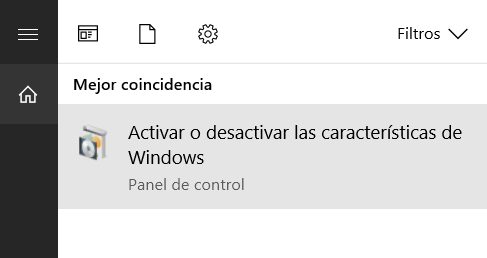
\includegraphics[width=8cm]{./Imagenes/1} 
\end{center}


\begin{itemize}
- Buscamos la opción llamada 'Hyper V', lo activamos la casilla y reiniciamos la pc.\\
\end{itemize}

\begin{center}
	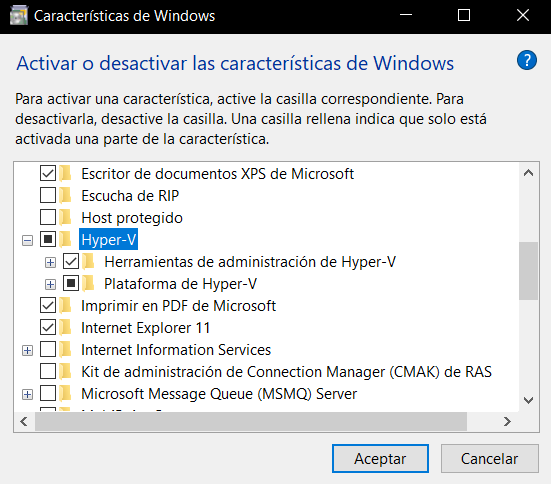
\includegraphics[width=8cm]{./Imagenes/2} 
\end{center}


\begin{itemize}
\subsection{Configuración del Hyper-V}\\
- Nos dirigimos a 'Administrador de conmutadores virtuales'. En la ventana que nos muestra
tenemos que elegir conmutador 'Interno', luego hacemos click en 'Crear conmutador virtual'.
\end{itemize}

\begin{center}
	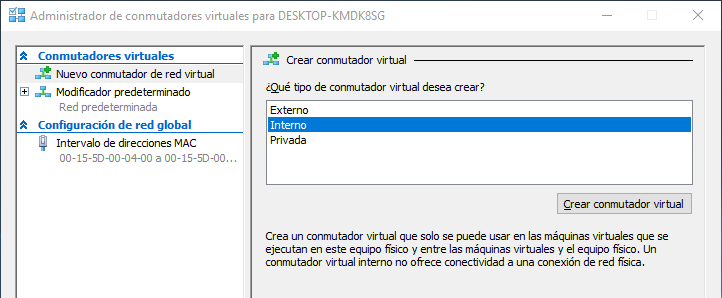
\includegraphics[width=10cm]{./Imagenes/3} 
\end{center}


\begin{itemize}
- Nos pedirá ingresar un nombre, ponemos el que deseamos. Verificamos si esta marcada la casilla
en 'Red interna' y damos click en 'Aceptar'.\\
\end{itemize}

\begin{center}
	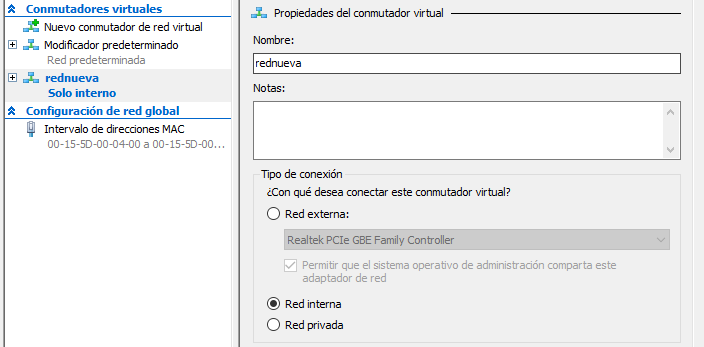
\includegraphics[width=10cm]{./Imagenes/4} 
\end{center}


\begin{itemize}
- Ingresamos a la opción 'Configuración de Hyper-V', le asignaremos una ruta donde se almacenará los archivos instalados.\\
\end{itemize}

\begin{center}
	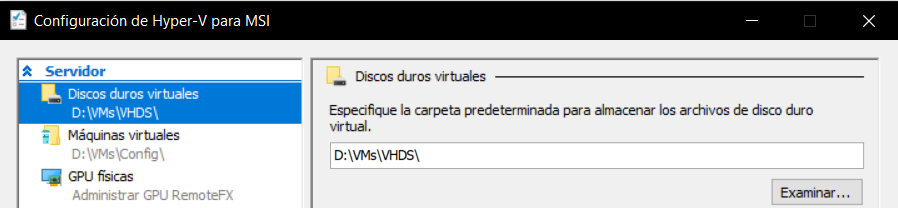
\includegraphics[width=12cm]{./Imagenes/5} 
\end{center}



\begin{itemize}
- Luego del mismo modo pasaremos a configurar la ruta donde se guardará la máquina virtual\\
\end{itemize}

\begin{center}
	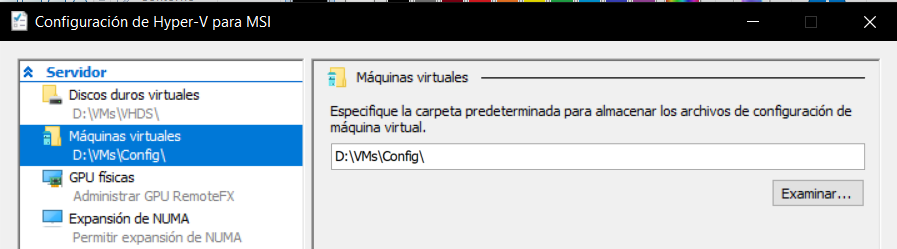
\includegraphics[width=12cm]{./Imagenes/6} 
\end{center}

\begin{itemize}

\subsection{Creación de la maquina virtual en Hyper-V}\\
- Hacemos click en 'Nuevo-Maquina virtual'. En la ventana que nos muestra ingresamos el nombre que deseemos poner a la maquina virtual, damos siguiente.
\end{itemize}

\begin{center}
	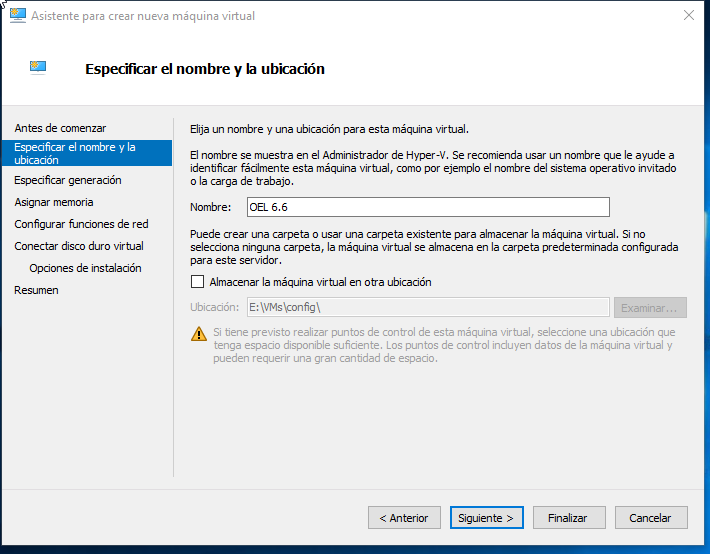
\includegraphics[width=10cm]{./Imagenes/7} 
\end{center}



\begin{itemize}
- Elegimos la generación por defecto\\
\end{itemize}

\begin{center}
	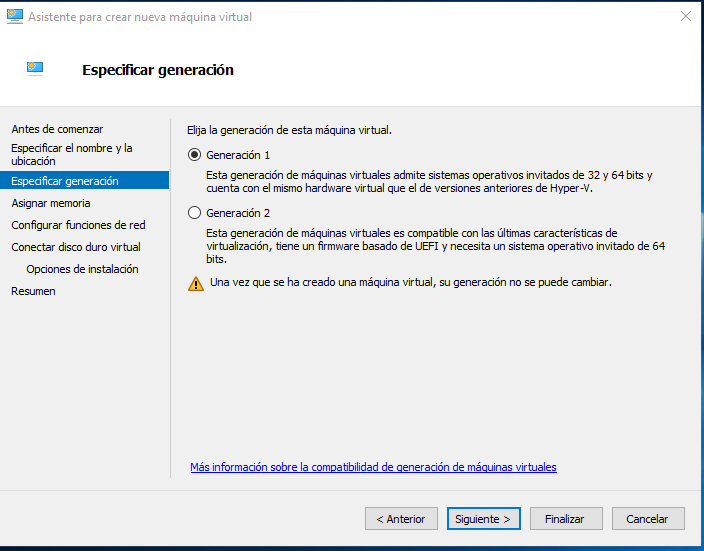
\includegraphics[width=12cm]{./Imagenes/8} 
\end{center}



\begin{itemize}
- Asignamos un total de 2048 MB de memoria RAM\\
\end{itemize}

\begin{center}
	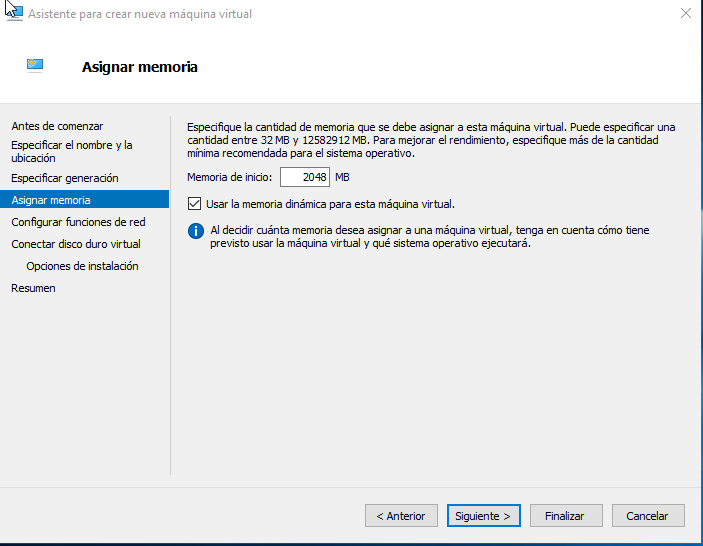
\includegraphics[width=12cm]{./Imagenes/9} 
\end{center}


\begin{itemize}
- En esta parte asignamos la red que hemos creado anteriormente, que en esta ocasión esta con el nombre de 'rednueva'\\
\end{itemize}

\begin{center}
	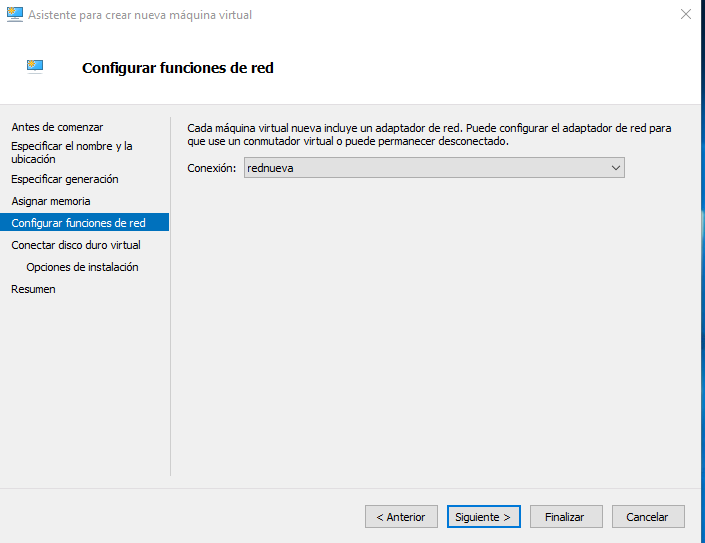
\includegraphics[width=12cm]{./Imagenes/10} 
\end{center}

\begin{itemize}
- En esta ventana escogemos la opción de 'Usar un disco
duro virtual existente', damos click en siguiente y finalizamos la instalación\\
\end{itemize}

\begin{center}
	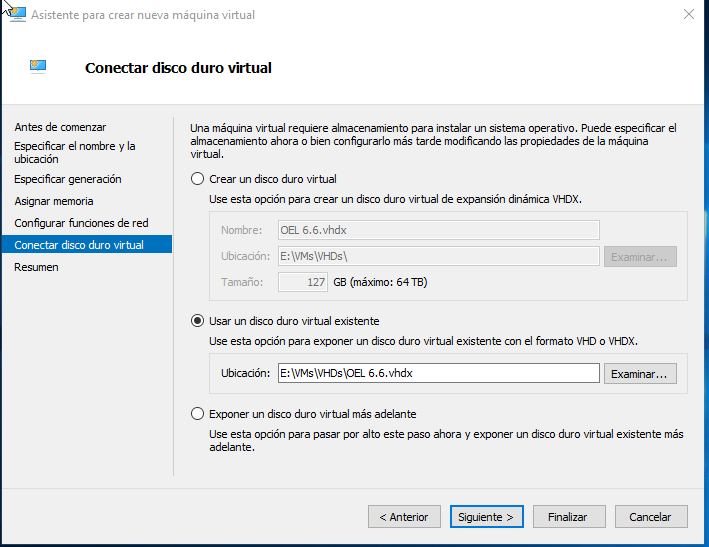
\includegraphics[width=12cm]{./Imagenes/11} 
\end{center}


\begin{itemize}
- Luego de ser creado la maquina virtual, lo seleccionamos y nos dirigimos a la pestaña de 'configuración'. Cambiaremos la opción de procesador y escogeremos a 2 el numero de procesadores. Damos click en aceptar\\
\end{itemize}

\begin{center}
	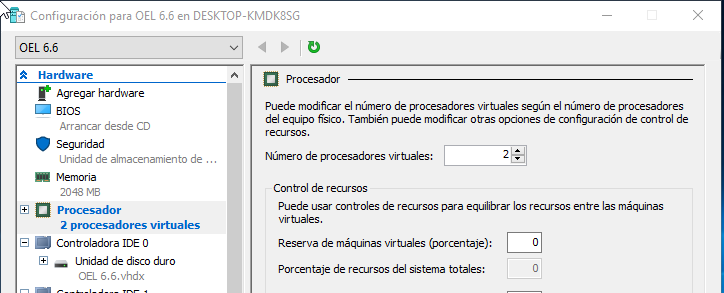
\includegraphics[width=12cm]{./Imagenes/12} 
\end{center}


\begin{itemize}
- Ahora iniciaremos la maquina virtual, escogemos la opción 'Iniciar' y luego 'Conectar'\\
\end{itemize}

\begin{center}
	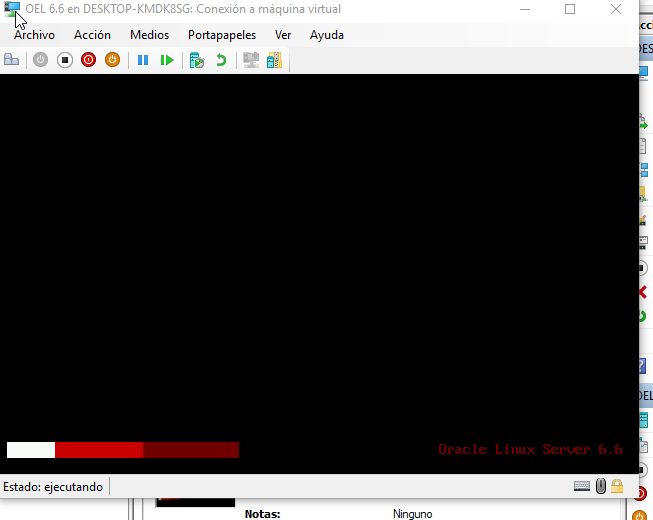
\includegraphics[width=12cm]{./Imagenes/13} 
\end{center}



\begin{itemize}
\subsection{Instalación de Oracle Database Server}\\
- En el sistema Operativo que hemos virtualizamos que en este caso es Oracle Linux, iniciamos sesion con el respectivo login y contraseña.
\end{itemize}

\begin{center}
	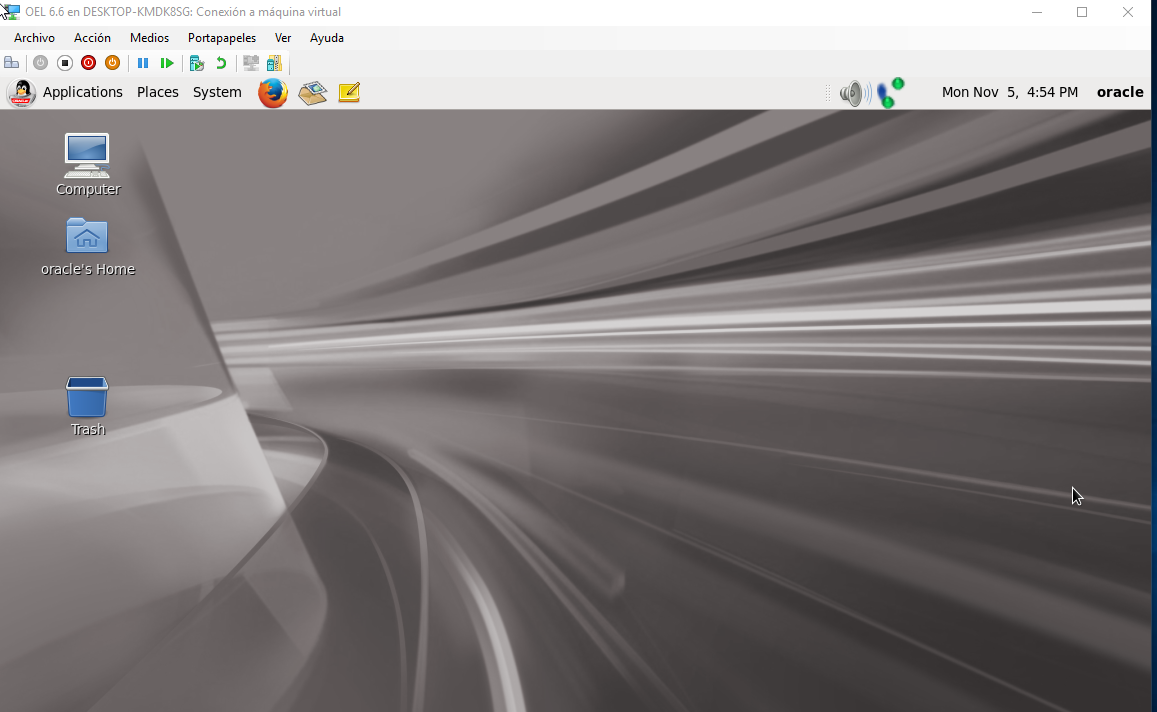
\includegraphics[width=10cm]{./Imagenes/14} 
\end{center}


\begin{itemize}
- Configuraremos las IPs tanto de la maquina virtual como del anfritrión. En la maquina real vamos a la opción 'conexiones de red' y seleccionamos la red que hemos creado al principio para el Hyper-V que esta con el nombre de 'rednueva'\\
\end{itemize}

\begin{center}
	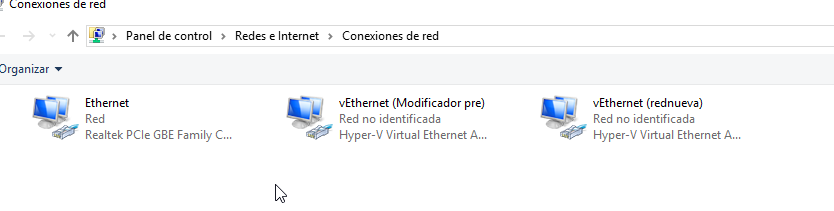
\includegraphics[width=12cm]{./Imagenes/15} 
\end{center}



\begin{itemize}
- Damos click en propiedades para poder cambiar el ip\\
\end{itemize}

\begin{center}
	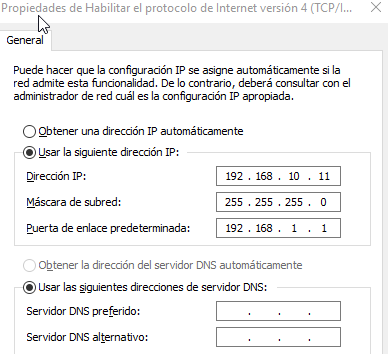
\includegraphics[width=12cm]{./Imagenes/16} 
\end{center}



\begin{itemize}
- Ahora en la maquina virtual en la parte superior hacemos click derecho y seleccionamos la opción 'Edit Connections'\\
\end{itemize}

\begin{center}
	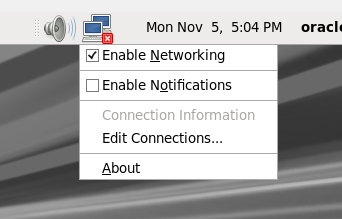
\includegraphics[width=12cm]{./Imagenes/17} 
\end{center}


\begin{itemize}
- Nos aparecerá dos opciones de lo cual borraremos el útimo, ahora editaremos el unico que ha quedado'\\
\end{itemize}

\begin{center}
	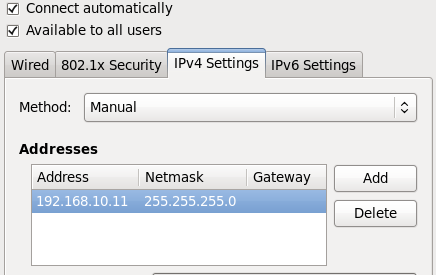
\includegraphics[width=12cm]{./Imagenes/18} 
\end{center}

\begin{itemize}
- Abrimos el terminal y agregamos los siguientes codigos para poder crear las carpetas necesarias\\
\end{itemize}

\begin{center}
	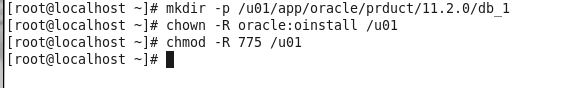
\includegraphics[width=12cm]{./Imagenes/19} 
\end{center}

\begin{itemize}
- Configuraremos algunos parámetros del kernel, para eso será necesario editar el archivo
/etc/sysctl.conf. Una vez dentro del archivo debemos añadir cietas lineas al final, quedando de esta manera\\
\end{itemize}

\begin{center}
	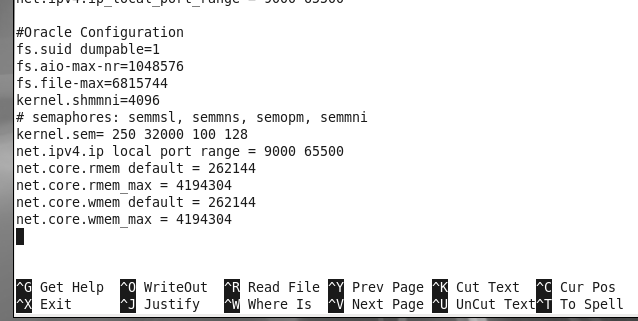
\includegraphics[width=12cm]{./Imagenes/20} 
\end{center}



\begin{itemize}
- Luego se debera realizar cambios a los limites de seguridad del sistema para el usuario, para lo
cual se debe editar el archivo /etc/security/limits.conf, una vez dentro del archivo configuramos de la siguiente manera\\
\end{itemize}

\begin{center}
	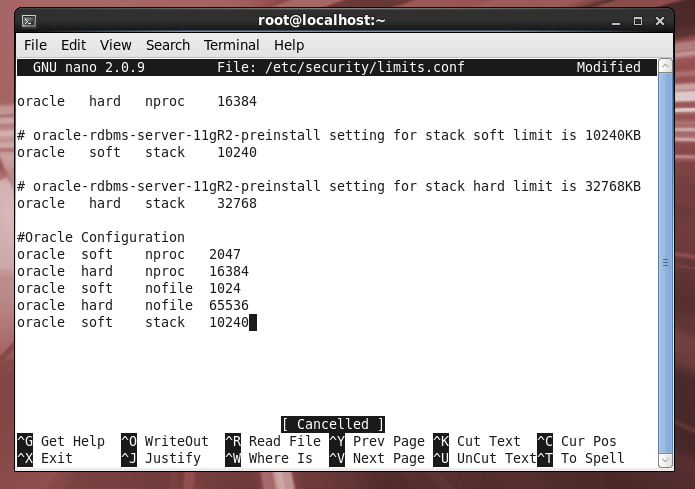
\includegraphics[width=12cm]{./Imagenes/21} 
\end{center}


\begin{itemize}
- Seguidamente escribimos el codigo ifconfig eth1\\
\end{itemize}

\begin{center}
	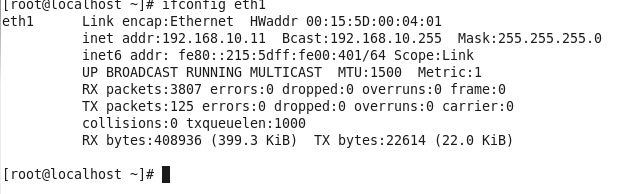
\includegraphics[width=12cm]{./Imagenes/22} 
\end{center}


\begin{itemize}
- Despues de establecer la dirección IP, debemos configurar el nombre del servidor, editamos el archivo /etc/host de la siguiente manera, luego reiniciamos la maquina virtual\\
\end{itemize}

\begin{center}
	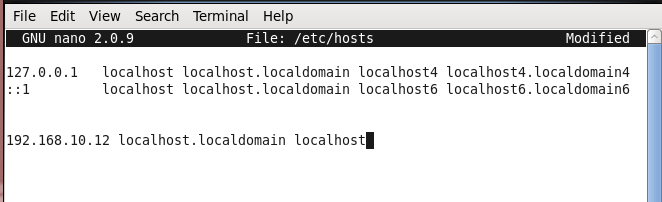
\includegraphics[width=12cm]{./Imagenes/23} 
\end{center}


\begin{itemize}
- Una vez reiniciado la maquina virtual, editamos el siguiente archivo .bash_profile, agregamos la siguiente configuracion y volvemos a reiniciar el sistema\\
\end{itemize}

\begin{center}
	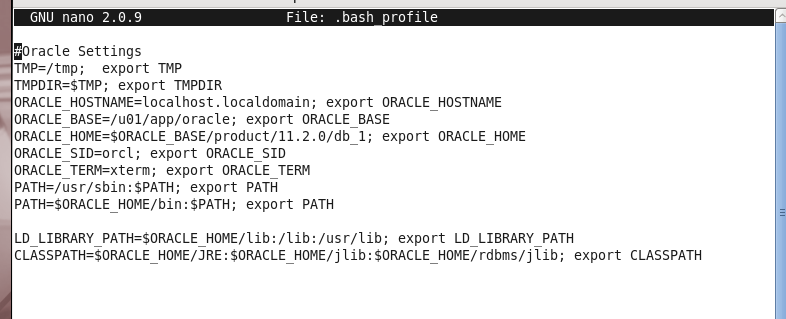
\includegraphics[width=12cm]{./Imagenes/24} 
\end{center}



\begin{itemize}
- Ahora descomprimimos los dos archivos zip, para poder ejecutar el instalador del Oracle\\
\end{itemize}

\begin{center}
	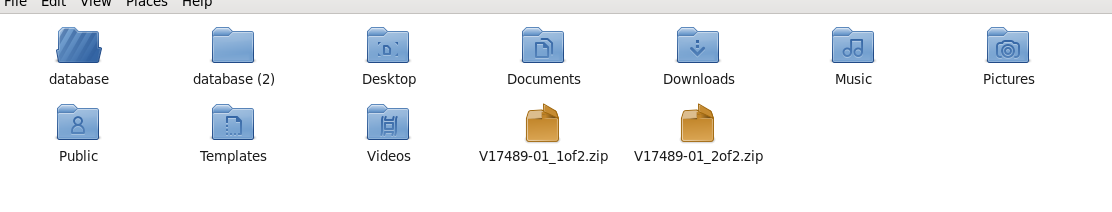
\includegraphics[width=12cm]{./Imagenes/25} 
\end{center}



\begin{itemize}
- Entramos a la carpeta database, hacemos click en runInstaller luego click en 'run in terminal'\\
\end{itemize}

\begin{center}
	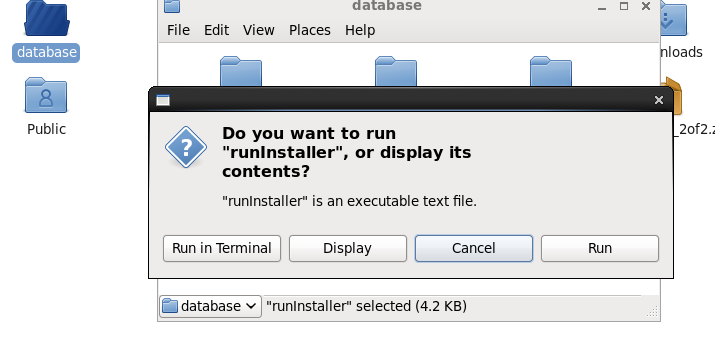
\includegraphics[width=12cm]{./Imagenes/26} 
\end{center}

\begin{itemize}
- Se abrirá el menú de instalación, escribiremos un correo y desmarcaremos el check, presionamos siguiente \\
\end{itemize}

\begin{center}
	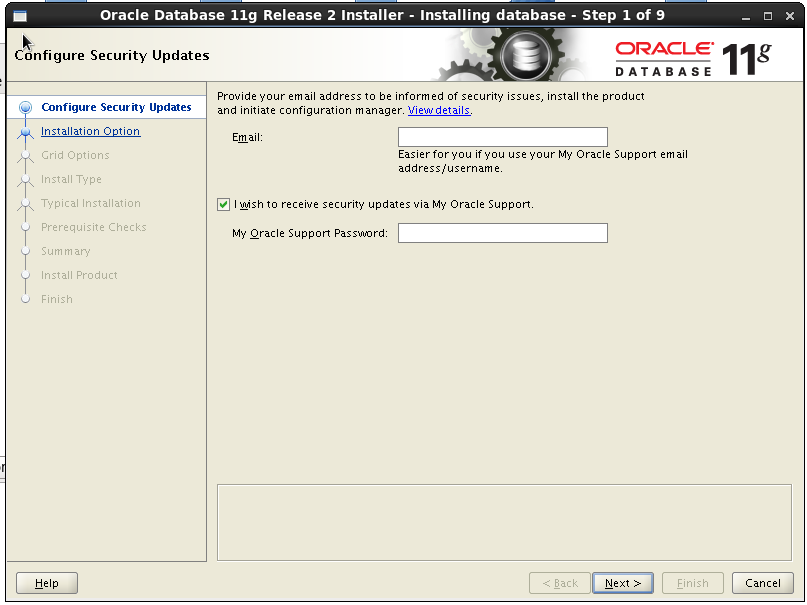
\includegraphics[width=12cm]{./Imagenes/27} 
\end{center}


\begin{itemize}
- Luego nos mostrará la siguiente imagen y selecciamos la primera opción  \\
\end{itemize}

\begin{center}
	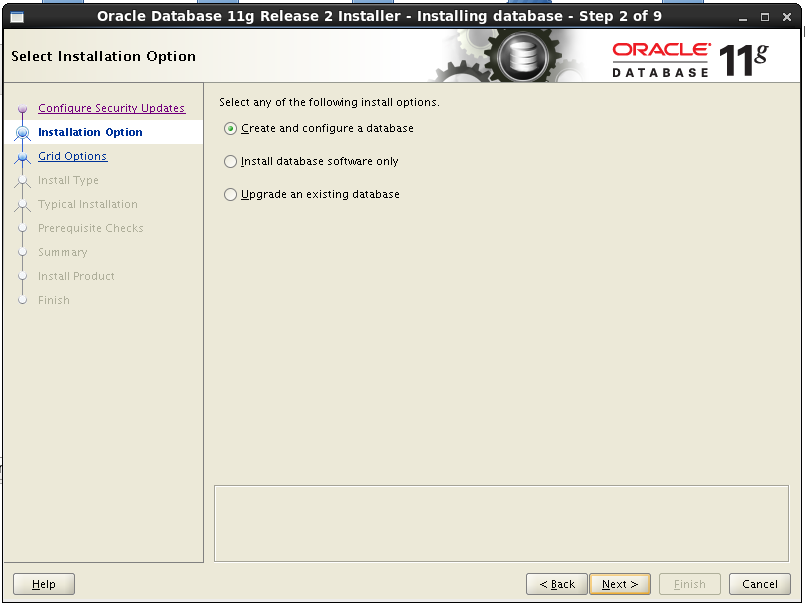
\includegraphics[width=12cm]{./Imagenes/28} 
\end{center}

\begin{itemize}
- Dejamos la opción marcado por defecto \\
\end{itemize}

\begin{center}
	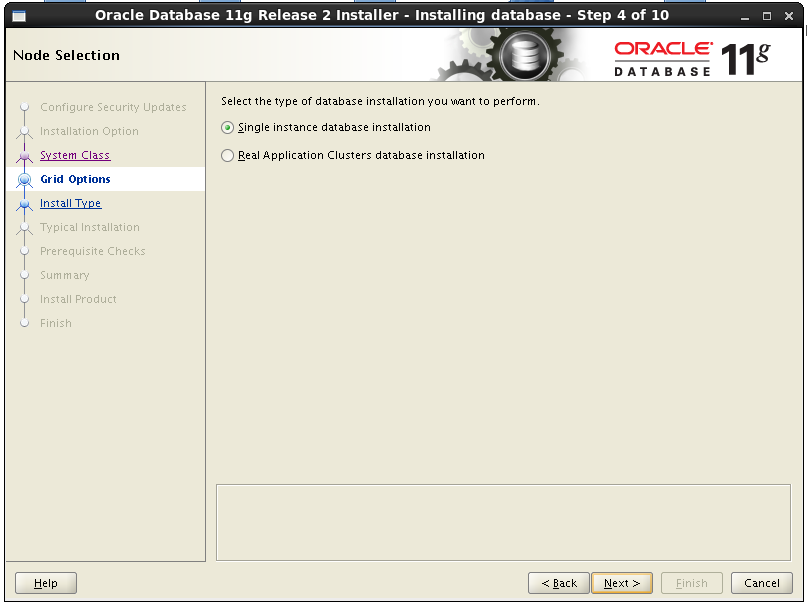
\includegraphics[width=12cm]{./Imagenes/29} 
\end{center}

\begin{itemize}
- En este paso dejamos marcado la opción por defecto, presionamos continuar \\
\end{itemize}

\begin{center}
	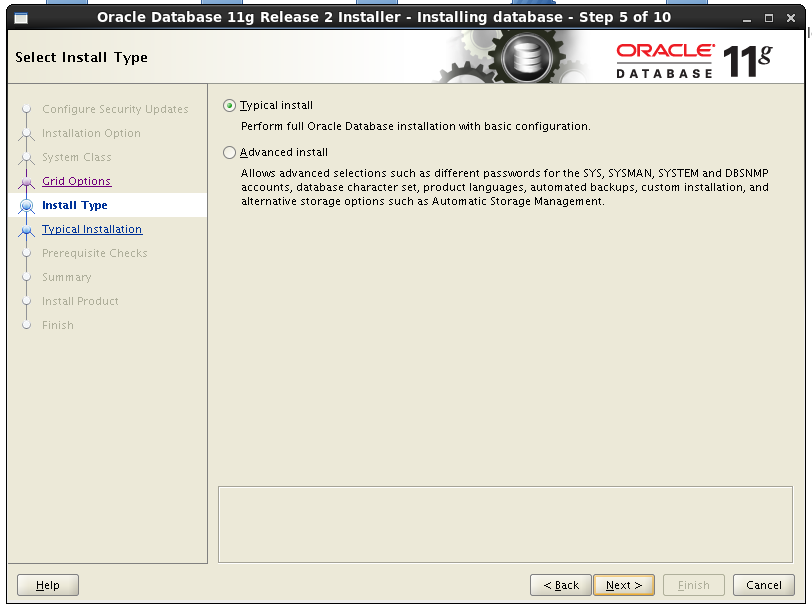
\includegraphics[width=12cm]{./Imagenes/30} 
\end{center}


\begin{itemize}
- Una vez llegado a este paso, tendremos que llenar datos necesarios para continuar \\
\end{itemize}

\begin{center}
	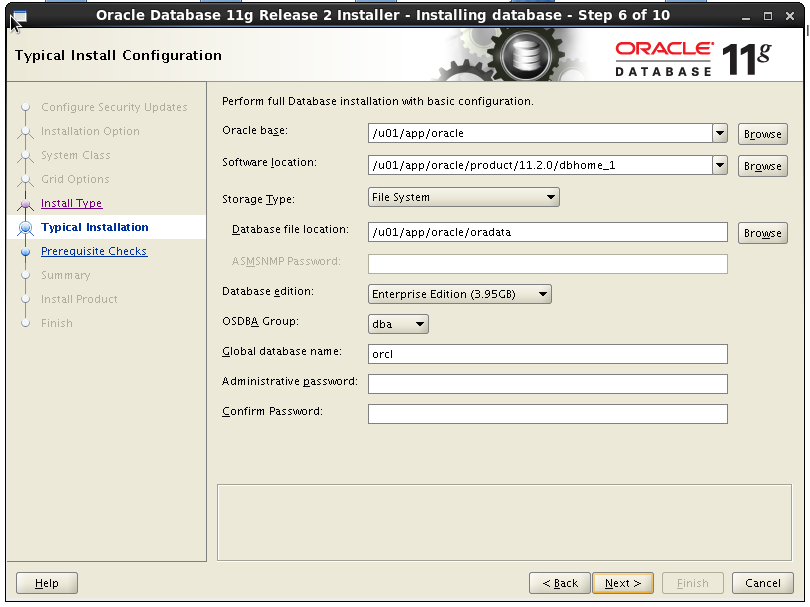
\includegraphics[width=12cm]{./Imagenes/31} 
\end{center}

\begin{itemize}
- Marcamos la casilla que esta en la esquina superior derecha, hacemos click en continuar \\
\end{itemize}

\begin{center}
	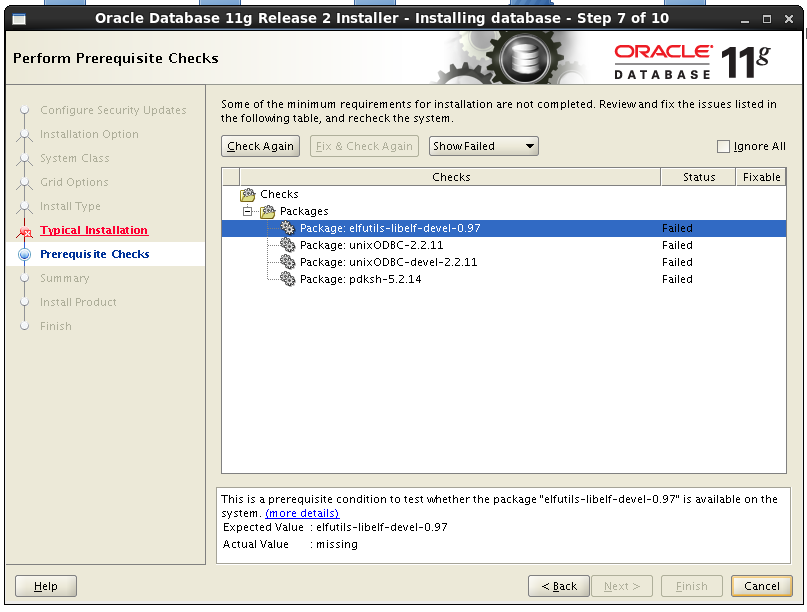
\includegraphics[width=12cm]{./Imagenes/32} 
\end{center}

\begin{itemize}
- Al terminar la instalación nos mostrará esta imagen \\
\end{itemize}

\begin{center}
	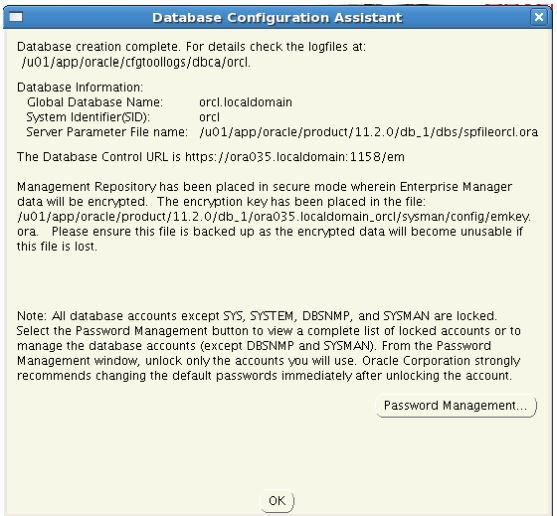
\includegraphics[width=12cm]{./Imagenes/33} 
\end{center}


\begin{itemize}
- Luego nos mostrará una ventan, cambiamos de usuario a root y copiamos las dos rutas en una terminal \\
\end{itemize}

\begin{center}
	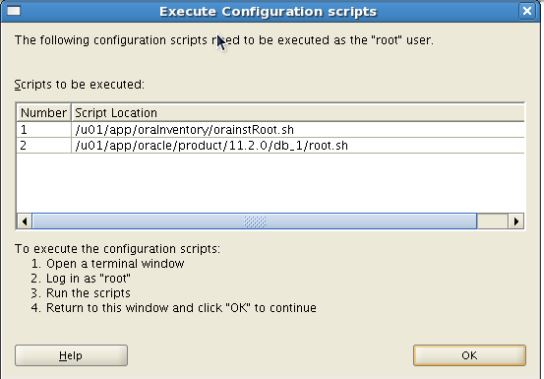
\includegraphics[width=12cm]{./Imagenes/34} 
\end{center}


\begin{itemize}
- Por ultimo abrimos un navegador, ponemos la siguiente dirección para poder ingresar al gestor de base de datos oracle \\
\end{itemize}

\begin{center}
	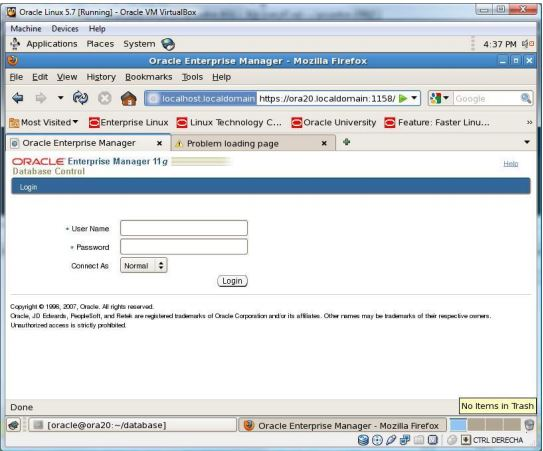
\includegraphics[width=12cm]{./Imagenes/35} 
\end{center}

\section{Cuestionario} 
\subsection{Los valores introducidos al archivo sysctl.conf ¿que representan?}\\
\textbf{fs.suid-dumpable}
\begin{itemize}
- Es para a volcados de núcleo, el valor 1 permite volcados de núcleo que pueden ser leídos por el propietario del proceso de dumping \\
\end{itemize}

\textbf{fs.aio-max-nr}
\begin{itemize}
- Es para establecer el aio-max-nrvalor, esto ayuda a HyperScale a tener un rendimiento óptimo. \\
\end{itemize}

\textbf{fs.file-max}
\begin{itemize}
- Establece el número máximo de manejadores de archivos que asignará el kernel de Linux. \\
\end{itemize}

\textbf{kernel.shmmni}
\begin{itemize}
- Establece el número máximo de segmentos de memoria compartida en todo el sistema. \\
\end{itemize}

\textbf{kernel.sem }
\begin{itemize}
- Establece parámetros de semáforo: SEMMSL, SEMMNS, SEMOPM y SEMMNI \\
\end{itemize}

\textbf{net.ipv4.ip-local-port-range}
\begin{itemize}
- Define el puerto mínimo y máximo que una conexión de red puede usar como su puerto de origen (local). \\
\end{itemize}

\textbf{net.core.rmem-default}
\begin{itemize}
- Un parámetro de kernel que controla el tamaño predeterminado de búferes de recepción utilizado por conectores. \\
\end{itemize}

\textbf{net.core.rmem-max }
\begin{itemize}
- Ajusta el máximo de bufer de recepción para todos los protocolos \\
\end{itemize}


\textbf{net.core.wmem-default }
\begin{itemize}
- Esto establece el tamaño del búfer de envío del sistema operativo predeterminado para todos los tipos de conexiones. \\
\end{itemize}

\textbf{net.core.wmem-max}
\begin{itemize}
- Ajusta el máximo de bufer de envio para todos los protocolos \\
\end{itemize}

\subsection{¿Con qué usuario(s) puedo conectarme al servidor a través del Administrador Empresarial?}\\
\begin{itemize}
- SYS y Oracle \\
\end{itemize}

\subsection{Capture una imagen de pantalla del navegador con el Administrador Empresarial, con el nombre de su servidor e iniciada la sesión del usuario SYS}\\

\begin{center}
	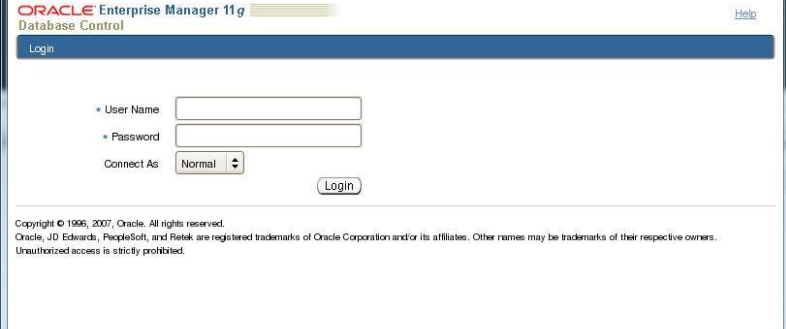
\includegraphics[width=12cm]{./Imagenes/36} 
\end{center}

\end{document}